\documentclass[]{article}
%\usepackage[latin1]{inputenc}
\usepackage[utf8]{inputenc}
\usepackage{float}
% Esto es para que el LaTeX sepa que el texto está en español:
%\usepackage[spanish]{babel}

% Paquetes de la AMS:
\usepackage{amsmath, amsthm, amsfonts}
\usepackage{graphicx}

%opening
\title{Trabajo Práctico 1}
\author{Jairo Jiménez \\
	Sergio De Raco}

\begin{document}

\maketitle


\section*{Objetivo}
El objetivo del presente trabajo es analizar las característcas en las cuáles el algoritmo J48 es robusto. El algoritmo será aplicado sobre la base de datos Latinobarómetro \cite{Latinobarometro2011}, la cual es una encuesta de percepción política, democrática y social de latinoamérica. Para poder observar las cualidades y deficiencias del algoritmo, este será sometido a diferentes tipos de pruebas para analizar su comportamiento.

\section*{Alcance}


\section*{Resultados esperados}
\begin{itemize}
	\item Confianza: Crecimiento en training, crecimiento en test hasta un valor de confianza particular, luego decrecimiento (Empieza el sobreajuste)
	\item Faltantes: Robustez cuando el árbol tiene pocos faltantes o faltantes sobre una sola variable. Decadencia cuando se aumenta la cantidad de faltantes sobre todas las variables, sobre ajuste cuando la imputación es hecha teniendo en cuenta la clase, en el caso contrario se espera poco poder predictivo.
	\item Ruido: Poco poder predictivo del árbol en la medida que la cantidad de Ruido aumenta.
	\item Discretización: Robustez cuando la variable numérica no es buen discriminador. Sobre ajuste cuando la variablee numérica adquiere poder predictivo.
\end{itemize}

\section*{Metodología}
Para la realización del presente trabajo, se pretende usar el sofware de minería de datos Weka \cite{Weka1} mediante el lenguaje estadístico R \cite{RCran} usando el paquete RWeka \cite{RWeka}

\section{Sobreajuste y poda}

El mejor ajuste del árbol se da cuando la confianza es de 0.1, después de este valor, empieza el sobreajuste del árbol, pues este deja baja la capacidad de pronosticar las nuevas instancias de manera correcta\\
A medida que aumenta la confianza, aumentan el tamaño y el número de hojas Figura \ref{1.P1Conf}

%\begin{figure}
%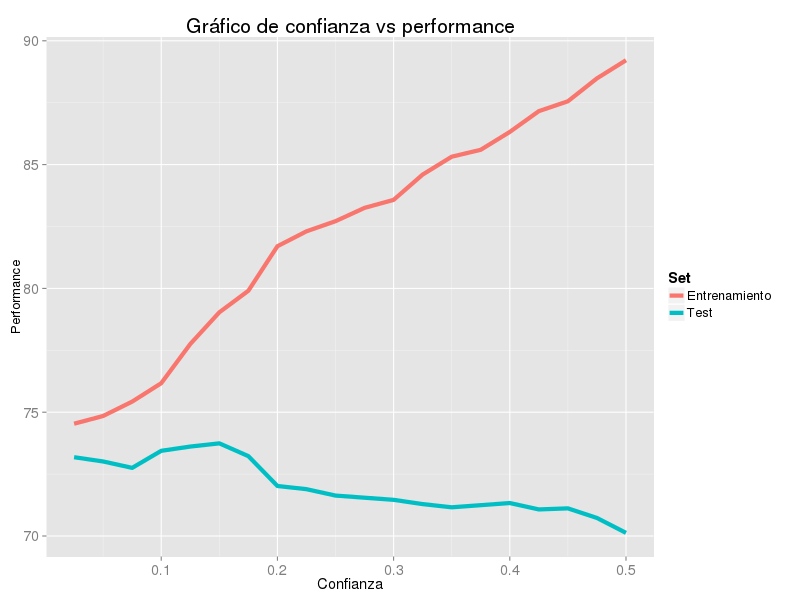
\includegraphics[width=0.8\linewidth,height=0.4\textheight]{Punto_1_Confianza_VS_ajuste}
%\caption[Confianza vs ajuste]{Confianza vs Ajuste}
%\label{P1ConfVSAjus}
%\end{figure}

\begin{figure}[H]
	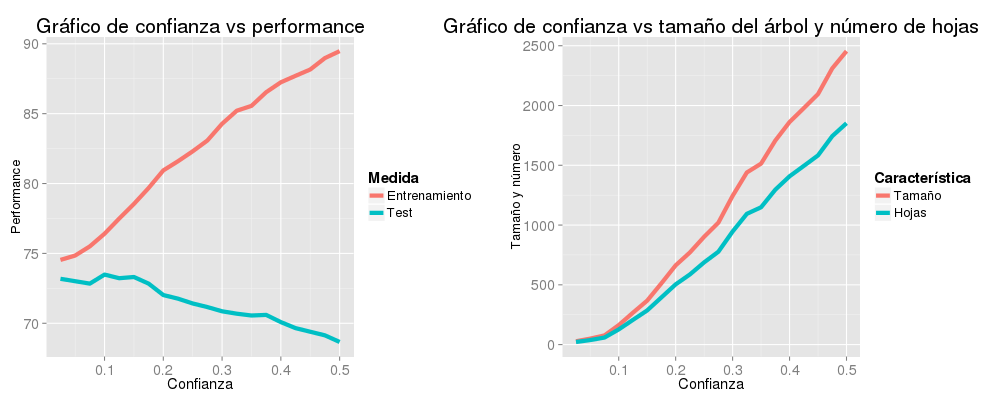
\includegraphics[scale = 0.4]{1_3_Conf_Perf_Num}
	\caption[Confianza vs ajuste]{Gráficos de confianza}
	\label{1.P1Conf}
\end{figure}
%
%
%\begin{figure}
%	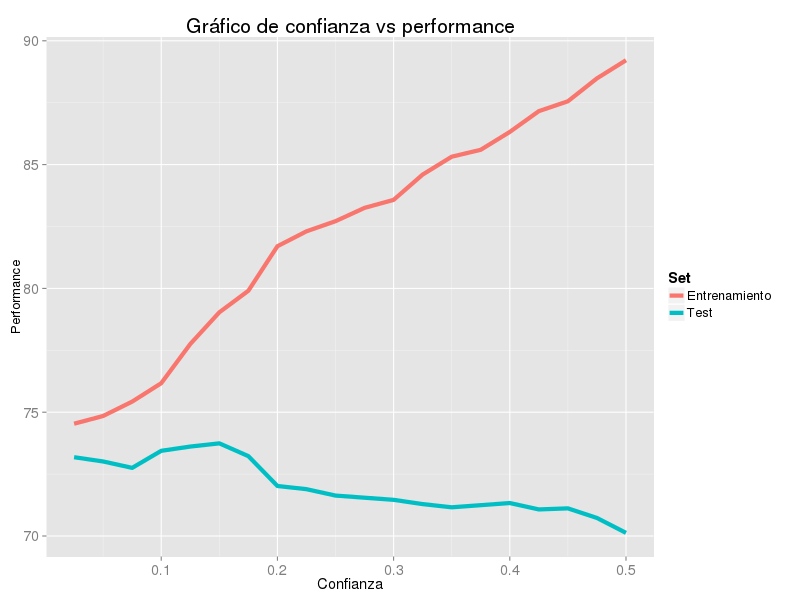
\includegraphics[scale = 0.4]{Punto_1_Confianza_VS_ajuste}
%	\caption[Confianza vs ajuste]{Confianza vs Ajuste}
%	\label{P1ConfVSAjus}
%\end{figure}

%\begin{figure}
%	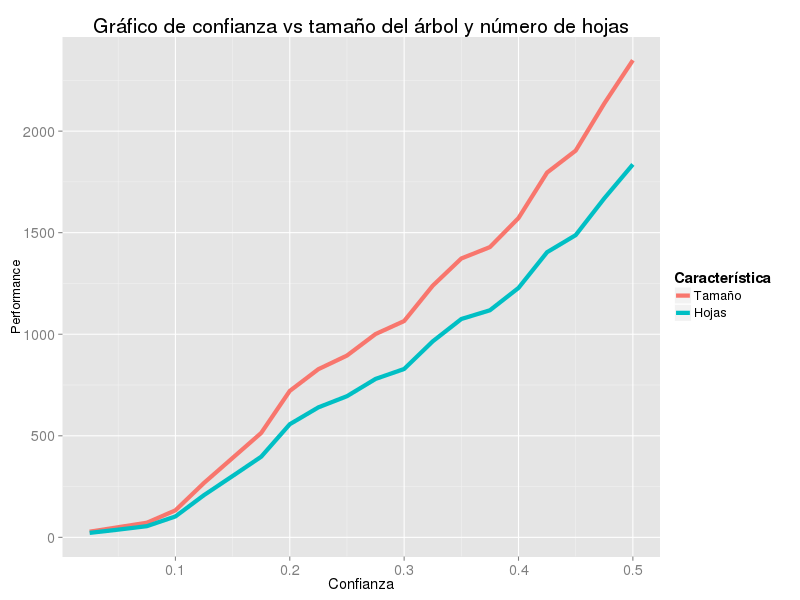
\includegraphics[scale = 0.4]{Punto_1_Confianza_VS_tamano}
%	\caption[Confianza vs ajuste]{Confianza vs Tamaño}
%	\label{P1ConfVSTamano}
%\end{figure}





\section{Tratamiento de datos faltantes}
Para el análisis de datos faltantes, el algoritmo se sometió a 3 diferentes tipos de faltantes sobre el conjunto de datos. Primero se anaklizó el efecto de los datos faltantes sobre una sola columna, luego sobre varias columnas pero solamente induciendo un faltante por fila y por último sobre varias columnas pero induciendo varios faltantes por fila. En los 3 casos, la cantidad de datos faltantes fue aumentando de 0 a 85\%

\subsection{Sobre una sola variable}
En el caso de una variable, se seleccionó como candidata la variable que separa mejor el árbol. A esta variable se le agregaron faltantes desde 0 a 85\% Figura \ref{2.P2Unic_Var}

\begin{figure}[H]
	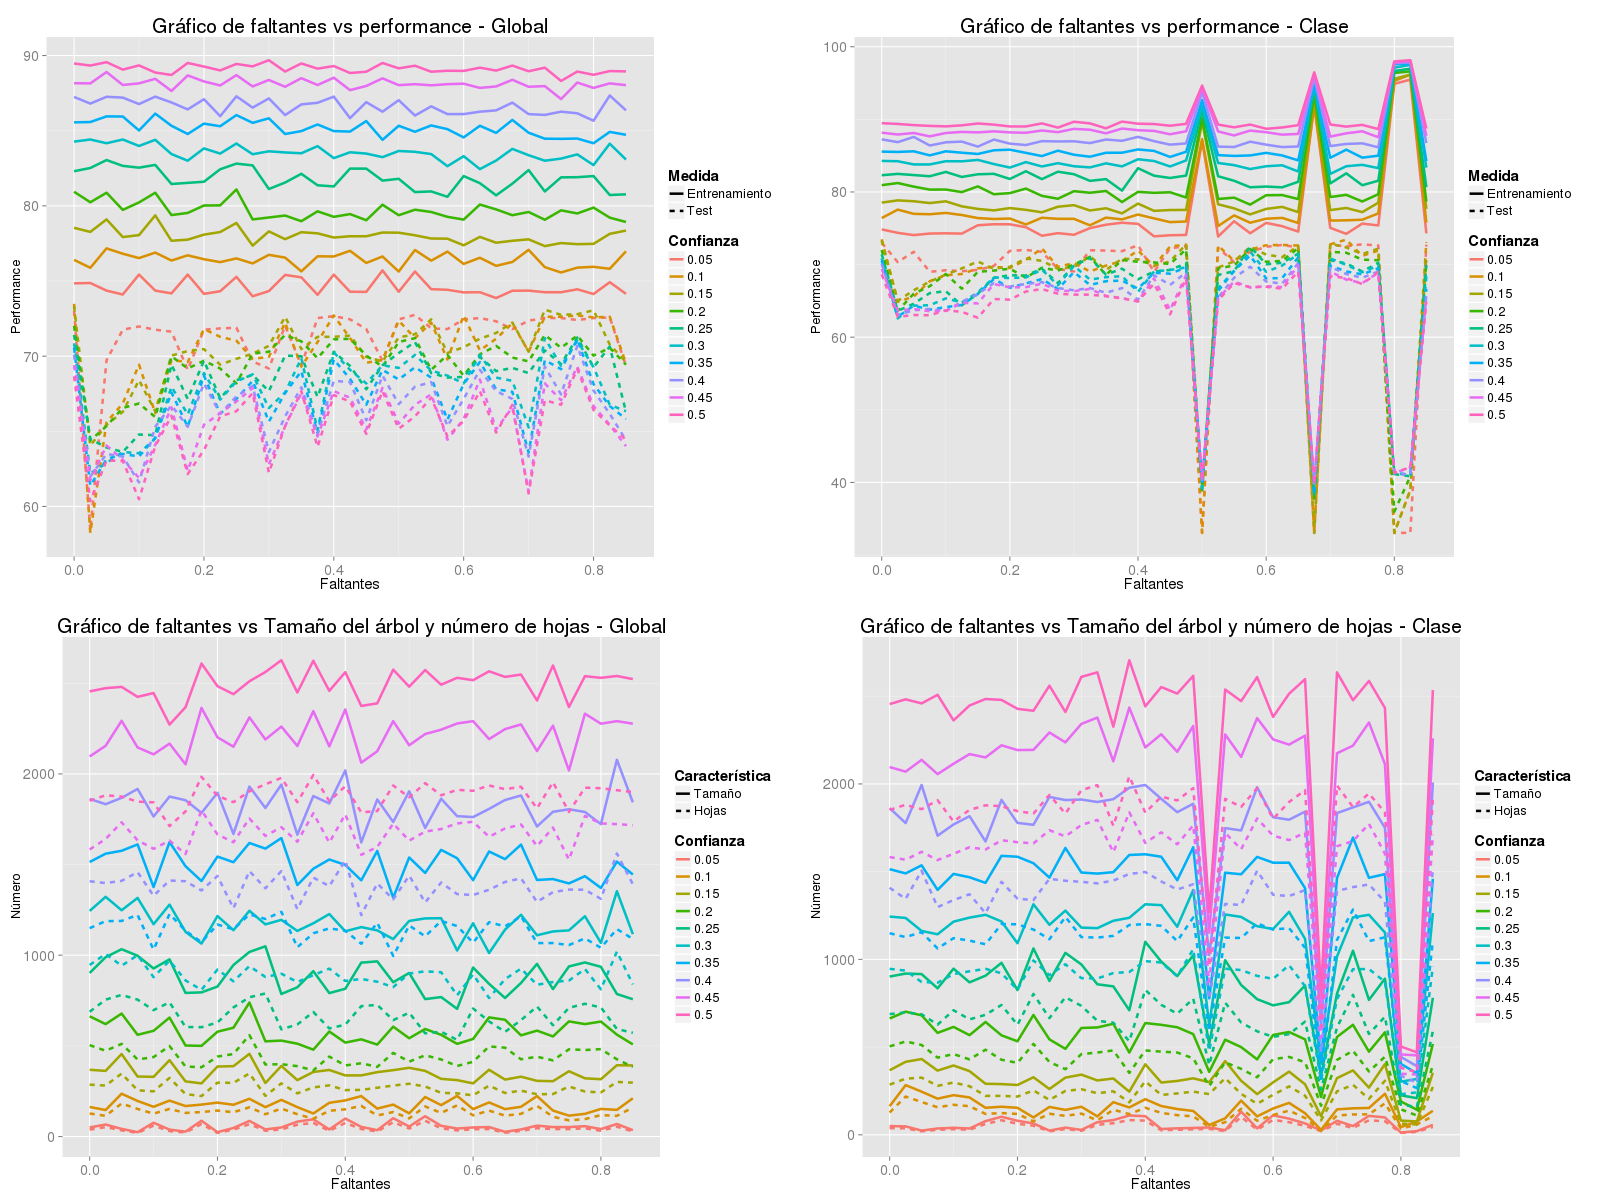
\includegraphics[scale = 0.27]{2_1_Unic_Col}
	\caption[Faltantes Unica variable]{Gráficos de Faltantes en una sola variable}
	\label{2.P2Unic_Var}
\end{figure}


\subsubsection{Imputación sin tener en cuenta la clase}

\subsubsection{Imputación teniendo en cuenta la clase}

\subsection{Sobre varias variables con un único faltante por fila}
En este caso, se agregaron datos faltantes de manera aleatoria a las columnas, pero tengiendo en cuenta que solamente se admite un valor faltante por fila en el conjunto de datos. Figura \ref{2.P2MultVarUnicFil} 

\begin{figure}[H]
	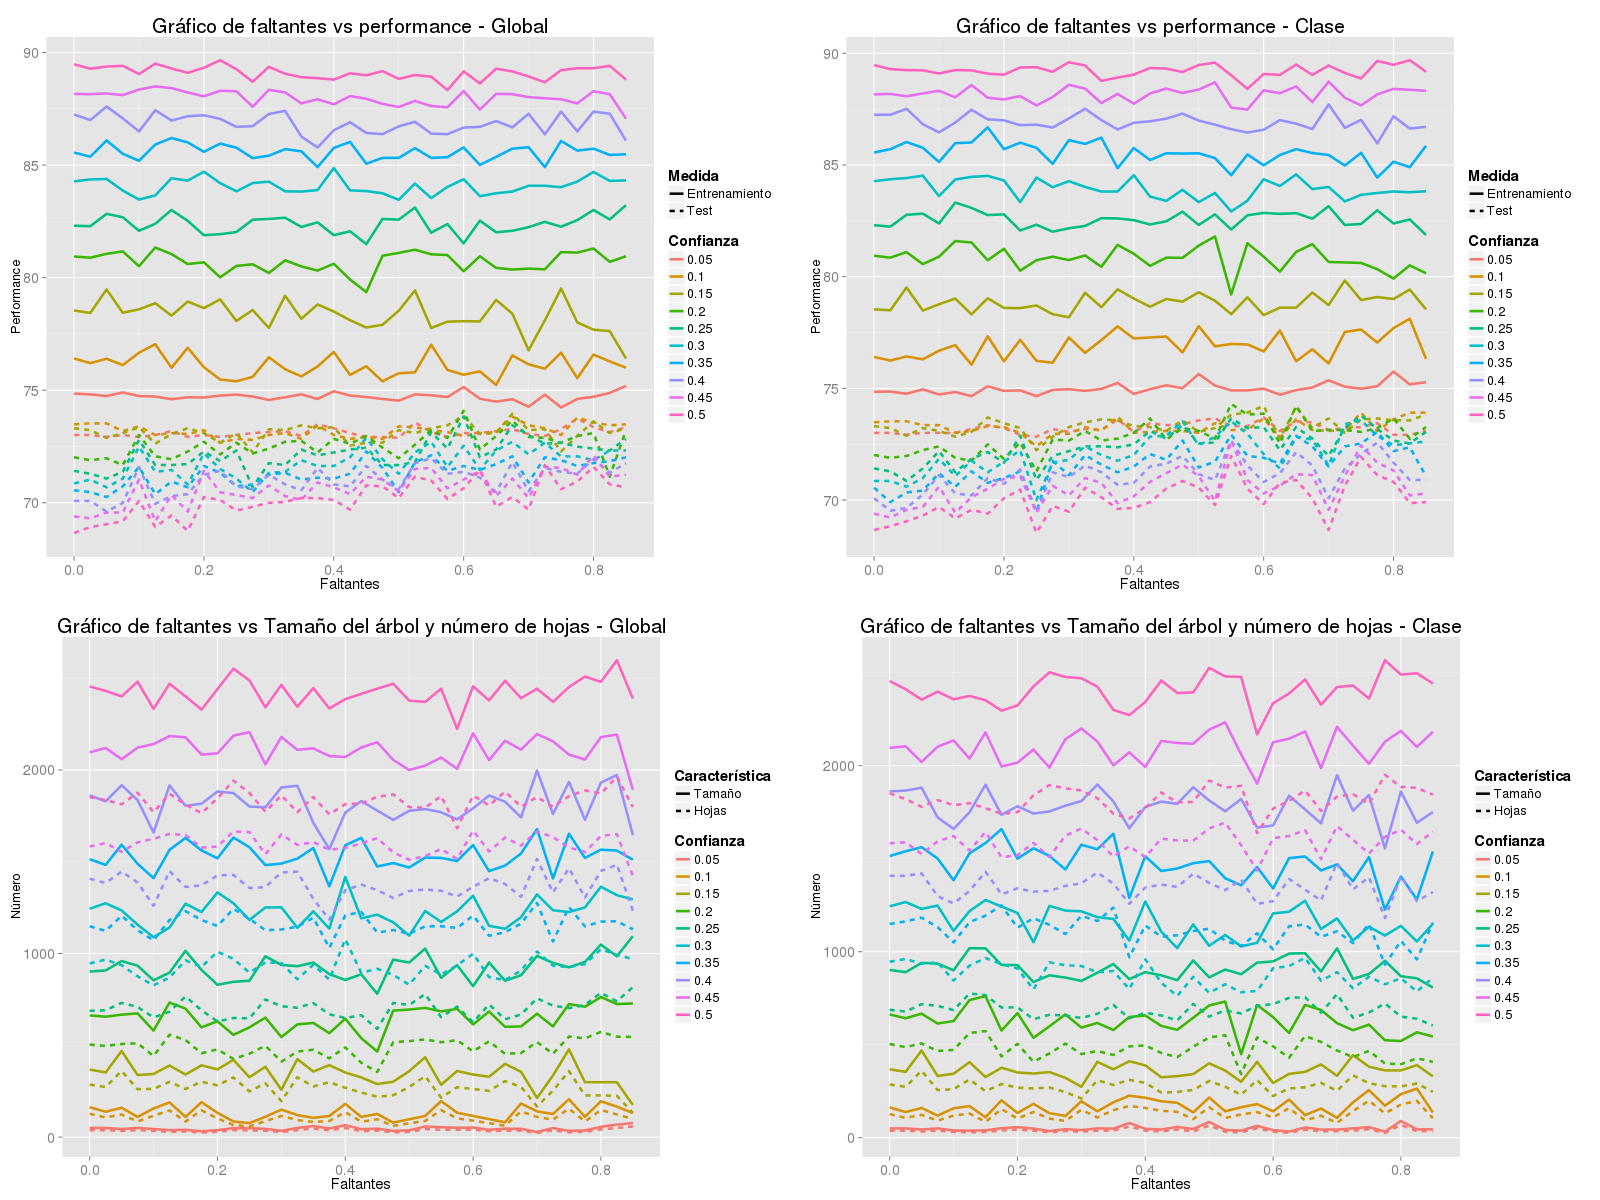
\includegraphics[scale = 0.27]{2_1_Mult_Col_Unic_Fil}
	\caption[Faltantes Múltiple variable]{Gráficos de Faltantes en Múltiples variables con un solo faltante por fila}
	\label{2.P2MultVarUnicFil}
\end{figure}

\subsubsection{Imputación sin tener en cuenta la clase}

\subsubsection{Imputación teniendo en cuenta la clase}

\subsection{Sobre varias variables con múltiples faltantes por fila}
Para el último análisis, se agregaron datos faltantes sobre el total de entradas de el conjunto de datos (total de filas por total de columnas). Figura \ref{1.P2MultVarMultFil}

\begin{figure}[H]
	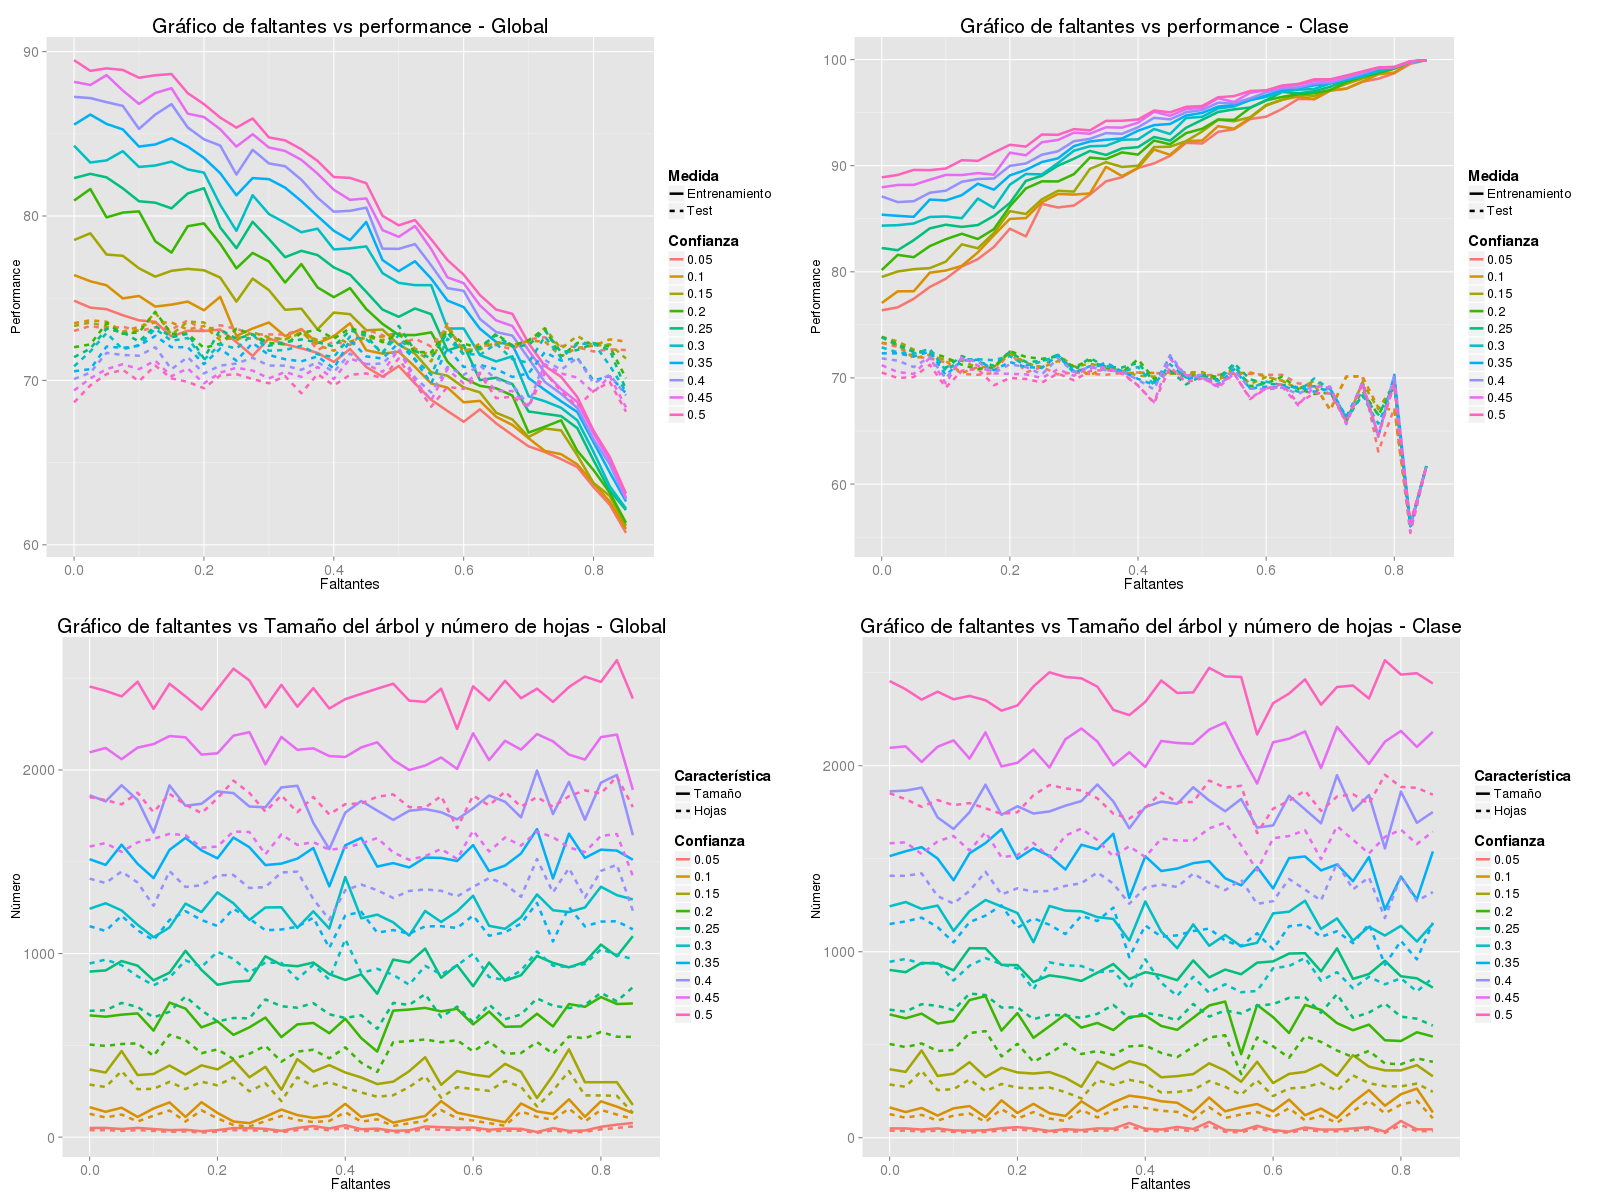
\includegraphics[scale = 0.27]{2_1_Mult_Col_Mult_Fil}
	\caption[[Faltantes Múltiples variables Múltiples Filas]{Gráficos de Faltantes en múltiples variables con múltiples faltantes por fila}
	\label{1.P2MultVarMultFil}
\end{figure}

\subsubsection{Imputación sin tener en cuenta la clase}

\subsubsection{Imputación teniendo en cuenta la clase}

\section{Tolerancia al ruido}
En esta parte, se genero entre 0 y 35\% de ruido sobre la clase. Figura \ref{3.P3Ruido}

\begin{figure}[H]
	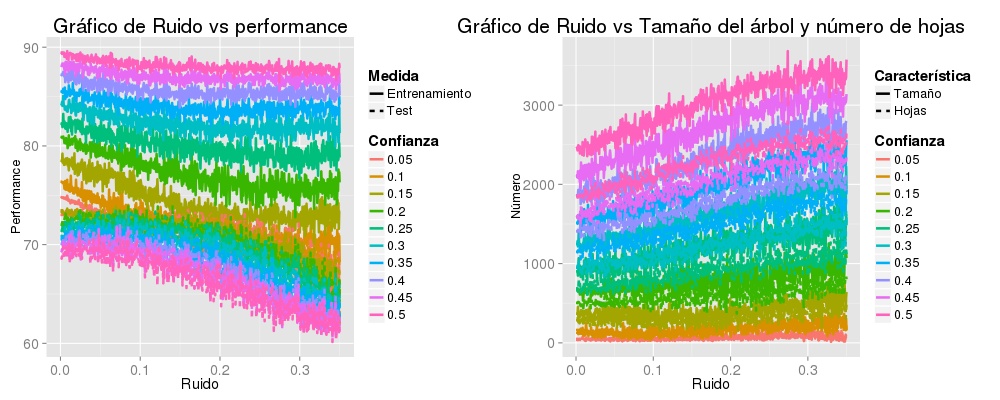
\includegraphics[scale = 0.4]{3_1_Ruido}
	\caption[Ruido]{Gráficos de Ruido}
	\label{3.P3Ruido}
\end{figure}

\section{Discretización de atributos numéricos}

\subsection{Sobre variables con poco poder discriminativo}

\subsection{Sobre variables con mucho poder discriminativo}

\section*{Conclusiones}
Con respecto a los datos faltantes, el árbol tiene una tolerancia similar a la mayoría de métodos estadísticos, en donde se admite al rededor de un 20\% de datos faltantes. 

\section*{Trabajo futuro}
Para poder verificar las propiedades del método para su aplicación en problemas de la vida real, sería conveniente mezclar las diferentes pruebas hechas sobre en este trabajo. ¿qué pasa cuando el árbol es sometido a ruido y a faltantes al mismo tiempo?. Además de esto, sería conveniente intentar otros métodos para imputación de datos categóricos que sesguen menos los datos, como por ejemplo el método de imputación Hot Deck, el cual, busca individuos similares al individuo con el dato faltante para "donarle" el dato que le hace falta. \cite{Rodgers1984}

\bibliographystyle{apalike}	
\bibliography{Bibliografia.bib}



%\section*{Referencias}

\end{document}
